\documentclass[a4paper]{article}\usepackage[]{graphicx}\usepackage[]{color}
%% maxwidth is the original width if it is less than linewidth
%% otherwise use linewidth (to make sure the graphics do not exceed the margin)
\makeatletter
\def\maxwidth{ %
  \ifdim\Gin@nat@width>\linewidth
    \linewidth
  \else
    \Gin@nat@width
  \fi
}
\makeatother

\definecolor{fgcolor}{rgb}{0.345, 0.345, 0.345}
\newcommand{\hlnum}[1]{\textcolor[rgb]{0.686,0.059,0.569}{#1}}%
\newcommand{\hlstr}[1]{\textcolor[rgb]{0.192,0.494,0.8}{#1}}%
\newcommand{\hlcom}[1]{\textcolor[rgb]{0.678,0.584,0.686}{\textit{#1}}}%
\newcommand{\hlopt}[1]{\textcolor[rgb]{0,0,0}{#1}}%
\newcommand{\hlstd}[1]{\textcolor[rgb]{0.345,0.345,0.345}{#1}}%
\newcommand{\hlkwa}[1]{\textcolor[rgb]{0.161,0.373,0.58}{\textbf{#1}}}%
\newcommand{\hlkwb}[1]{\textcolor[rgb]{0.69,0.353,0.396}{#1}}%
\newcommand{\hlkwc}[1]{\textcolor[rgb]{0.333,0.667,0.333}{#1}}%
\newcommand{\hlkwd}[1]{\textcolor[rgb]{0.737,0.353,0.396}{\textbf{#1}}}%
\let\hlipl\hlkwb

\usepackage{framed}
\makeatletter
\newenvironment{kframe}{%
 \def\at@end@of@kframe{}%
 \ifinner\ifhmode%
  \def\at@end@of@kframe{\end{minipage}}%
  \begin{minipage}{\columnwidth}%
 \fi\fi%
 \def\FrameCommand##1{\hskip\@totalleftmargin \hskip-\fboxsep
 \colorbox{shadecolor}{##1}\hskip-\fboxsep
     % There is no \\@totalrightmargin, so:
     \hskip-\linewidth \hskip-\@totalleftmargin \hskip\columnwidth}%
 \MakeFramed {\advance\hsize-\width
   \@totalleftmargin\z@ \linewidth\hsize
   \@setminipage}}%
 {\par\unskip\endMakeFramed%
 \at@end@of@kframe}
\makeatother

\definecolor{shadecolor}{rgb}{.97, .97, .97}
\definecolor{messagecolor}{rgb}{0, 0, 0}
\definecolor{warningcolor}{rgb}{1, 0, 1}
\definecolor{errorcolor}{rgb}{1, 0, 0}
\newenvironment{knitrout}{}{} % an empty environment to be redefined in TeX

\usepackage{alltt}
\usepackage[margin=1in]{geometry}
\IfFileExists{upquote.sty}{\usepackage{upquote}}{}
\begin{document}
% ---- Beginn Analysis -----
  \begin{center}
\section*{Analysis of Pixel-Wise Correlations}
\end{center}
So far we've only looked at the mean stain levels between different patients. However, this ignores any spatial processes that might play a role. In order to start gaining a first insight into what spatial processes might play a role we'll here analyse the pixel-wise correlation matrices for the cores from different patients. This will for example highlight the presence/absence of specific cell types/meta-phenotypes.

% =======================================================
\section{A First Look at the Data}
I compute the correlation matrices using python and save the lower triangular parts of these matrices to file. In order to adjust for the different scales of the stains  I calculate the standardised correlations using the \texttt{np.corrcoef()} function.

Let's load in the results and label the columns with the correlation they measure:
\begin{knitrout}
\definecolor{shadecolor}{rgb}{0.969, 0.969, 0.969}\color{fgcolor}\begin{kframe}
\begin{alltt}
\hlstd{corrArr} \hlkwb{=} \hlkwd{read.csv}\hlstd{(}\hlstr{"pixelcorrelations.csv"}\hlstd{,}\hlkwc{header}\hlstd{=F)}
\hlkwd{dim}\hlstd{(corrArr)}
\end{alltt}
\begin{verbatim}
## [1] 121 668
\end{verbatim}
\begin{alltt}
\hlcom{# Label the columns}
\hlstd{labelArr} \hlkwb{=} \hlkwd{c}\hlstd{(}\hlstr{"CoreId"}\hlstd{,}\hlstr{"PtSnty"}\hlstd{)}
\hlstd{markerLabelsVec} \hlkwb{=} \hlkwd{c}\hlstd{(}\hlstr{'SrBCK'}\hlstd{,} \hlstr{'RR101'}\hlstd{,} \hlstr{'RR102'}\hlstd{,} \hlstr{'AvantiLipid'}\hlstd{,} \hlstr{'XeBCK'}\hlstd{,} \hlstr{'CD196'}\hlstd{,} \hlstr{'CD19'}\hlstd{,} \hlstr{'Vimentin'}\hlstd{,}
                    \hlstr{'CD163'}\hlstd{,} \hlstr{'CD20'}\hlstd{,} \hlstr{'CD16'}\hlstd{,} \hlstr{'CD25'}\hlstd{,} \hlstr{'p53'}\hlstd{,} \hlstr{'CD134'}\hlstd{,} \hlstr{'CD45'}\hlstd{,} \hlstr{'CD44s'}\hlstd{,} \hlstr{'CD14'}\hlstd{,} \hlstr{'FoxP3'}\hlstd{,}
                    \hlstr{'CD4'}\hlstd{,} \hlstr{'E-cadherin'}\hlstd{,} \hlstr{'p21'}\hlstd{,} \hlstr{'CD152'}\hlstd{,} \hlstr{'CD8a'}\hlstd{,} \hlstr{'CD11b'}\hlstd{,} \hlstr{'Beta-catenin'}\hlstd{,} \hlstr{'B7-H4'}\hlstd{,} \hlstr{'Ki67'}\hlstd{,}
                    \hlstr{'CollagenI'}\hlstd{,} \hlstr{'CD3'}\hlstd{,} \hlstr{'CD68'}\hlstd{,} \hlstr{'PD-L2'}\hlstd{,} \hlstr{'B7-H3'}\hlstd{,} \hlstr{'HLA-DR'}\hlstd{,} \hlstr{'pS6'}\hlstd{,} \hlstr{'HistoneH3'}\hlstd{,} \hlstr{'DNA191'}\hlstd{,}
                    \hlstr{'DNA193'}\hlstd{)}
\hlkwa{for} \hlstd{(i} \hlkwa{in} \hlkwd{seq}\hlstd{(}\hlnum{2}\hlstd{,}\hlnum{37}\hlstd{)) \{}
  \hlkwa{for} \hlstd{(j} \hlkwa{in} \hlkwd{seq}\hlstd{(i}\hlopt{-}\hlnum{1}\hlstd{)) \{}
    \hlstd{labelArr} \hlkwb{=} \hlkwd{c}\hlstd{(labelArr,}\hlkwd{paste0}\hlstd{(markerLabelsVec[i],}\hlstr{":"}\hlstd{,markerLabelsVec[j]))}
  \hlstd{\}}
\hlstd{\}}
\hlkwd{names}\hlstd{(corrArr)} \hlkwb{=} \hlstd{labelArr}
\end{alltt}
\end{kframe}
\end{knitrout}

Let's compute the difference in the mean matrix of the responders and the non-responders and visualise it to see if there are any obvious differences

\begin{knitrout}
\definecolor{shadecolor}{rgb}{0.969, 0.969, 0.969}\color{fgcolor}\begin{kframe}
\begin{alltt}
\hlkwd{library}\hlstd{(ggplot2)}
\hlkwd{library}\hlstd{(reshape2)}
\hlstd{corrArr} \hlkwb{=} \hlstd{corrArr[}\hlkwd{with}\hlstd{(corrArr,} \hlkwd{order}\hlstd{(PtSnty)), ]}
\hlstd{corrArr} \hlkwb{=} \hlkwd{data.frame}\hlstd{(corrArr,}\hlkwc{LinId}\hlstd{=}\hlkwd{seq}\hlstd{(}\hlkwd{nrow}\hlstd{(corrArr)))}
\hlstd{corrArr_reshaped} \hlkwb{=} \hlkwd{melt}\hlstd{(corrArr[,}\hlopt{-}\hlnum{1}\hlstd{],}\hlkwc{id.vars}\hlstd{=}\hlkwd{c}\hlstd{(}\hlstr{"LinId"}\hlstd{))}
\hlkwd{ggplot}\hlstd{(corrArr_reshaped,} \hlkwd{aes}\hlstd{(variable, LinId))} \hlopt{+}
  \hlkwd{geom_tile}\hlstd{(}\hlkwd{aes}\hlstd{(}\hlkwc{fill} \hlstd{= value),}\hlkwc{colour}\hlstd{=}\hlstr{"white"}\hlstd{)} \hlopt{+}
  \hlkwd{scale_fill_gradient}\hlstd{(}\hlkwc{low}\hlstd{=}\hlstr{"white"}\hlstd{,}\hlkwc{high}\hlstd{=}\hlstr{"steelblue"}\hlstd{)} \hlopt{+}
  \hlkwd{theme_bw}\hlstd{()} \hlopt{+}
  \hlkwd{labs}\hlstd{(}\hlkwc{x}\hlstd{=}\hlstr{""}\hlstd{,}\hlkwc{y}\hlstd{=}\hlstr{"Core"}\hlstd{)} \hlopt{+}
  \hlkwd{theme}\hlstd{(}\hlkwc{axis.text.x} \hlstd{=} \hlkwd{element_text}\hlstd{(}\hlkwc{angle}\hlstd{=}\hlnum{90}\hlstd{,} \hlkwc{hjust}\hlstd{=}\hlnum{1}\hlstd{))}
\end{alltt}
\end{kframe}\begin{figure}[h]
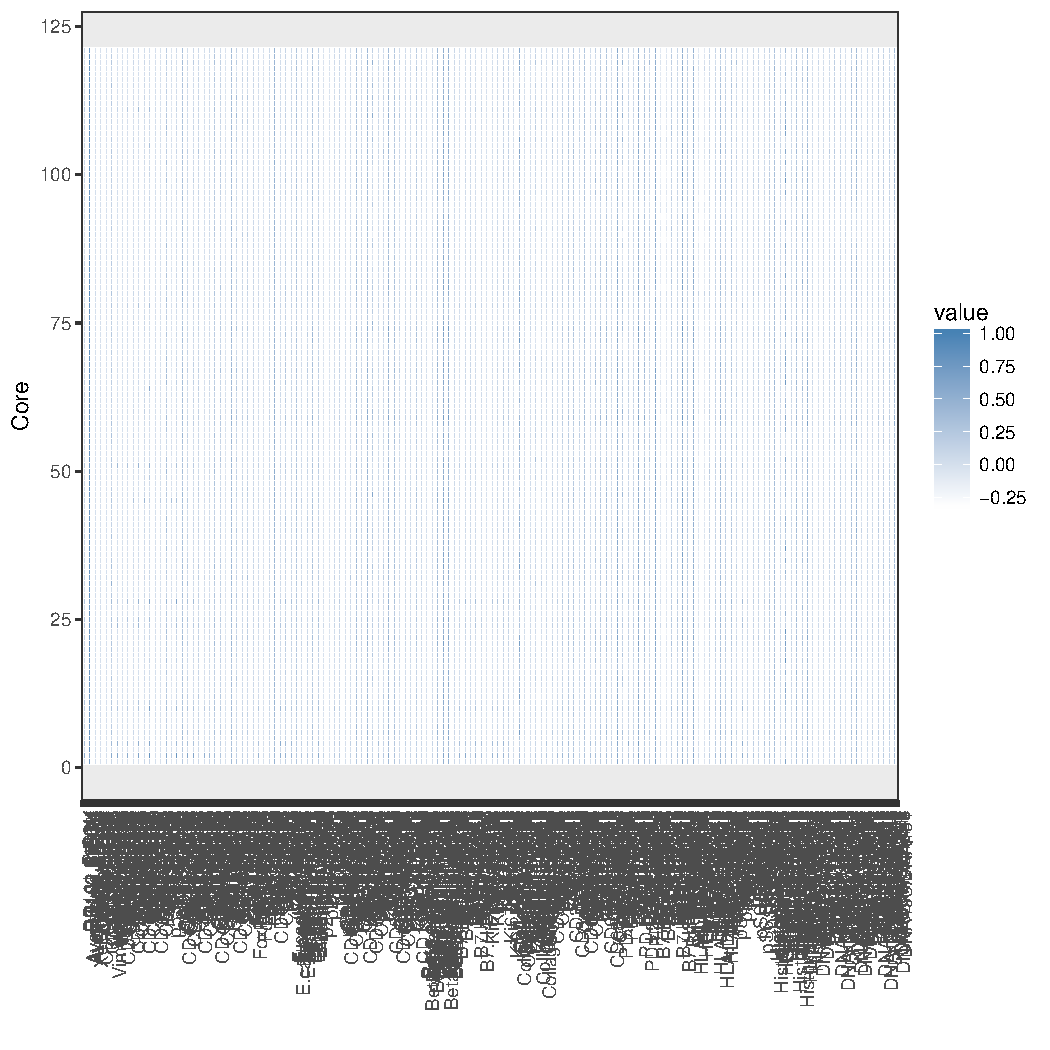
\includegraphics[width=\maxwidth]{figure/Fig_CorrMatrices-1} \caption[Pixel-wise correlation of the different stains for responders (top-half) and non-responders (bottom-half)]{Pixel-wise correlation of the different stains for responders (top-half) and non-responders (bottom-half).}\label{fig:Fig_CorrMatrices}
\end{figure}


\end{knitrout}
  

\end{document}
